\section{Luồng dữ liệu}
Hệ thống được tổ chức theo luồng dữ liệu xuyên suốt từ khâu thu thập cho đến khi phục vụ người dùng cuối. Dữ liệu giao thông (video, hình ảnh, thông tin cảm biến, v.v.) chảy qua các tầng kiến trúc như sau, đảm bảo khả năng xử lý theo thời gian thực và phân tích dự báo.
\begin{figure}[H]
    \centering
    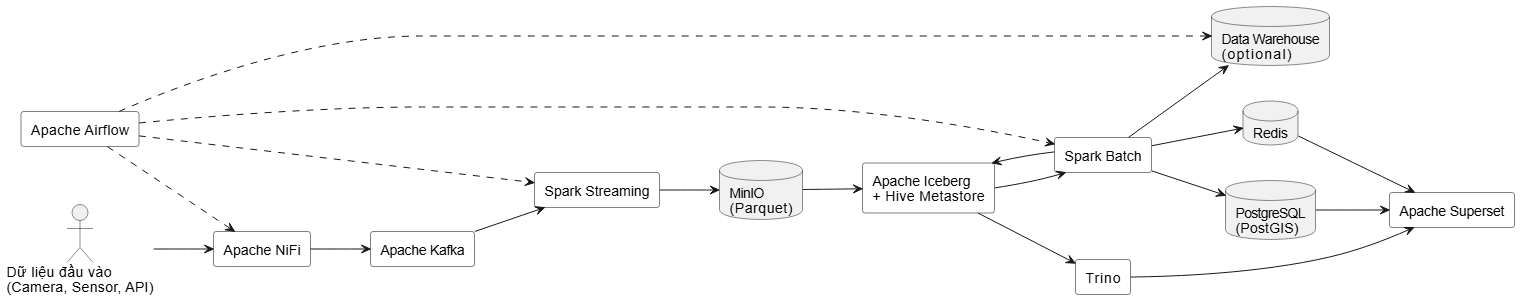
\includegraphics[width=\linewidth]{Images/dataflow.png}
    \caption{Luồng dữ liệu}
    \label{fig:enter-label}
\end{figure}
\subsection{Thu thập và truyền tải dữ liệu (Ingestion)}
Dữ liệu từ camera, cảm biến và API được thu thập và đưa vào hệ thống thông qua Apache NiFi. NiFi kết nối đến các nguồn dữ liệu thô, thực hiện chuẩn hóa định dạng và định tuyến luồng dữ liệu đa cấu trúc này. Tiếp đó, NiFi ingest dữ liệu vào Apache Kafka – một nền tảng streaming phân tán – đóng vai trò như “bus” truyền thông điệp theo thời gian thực. Kafka bảo đảm việc truyền tải dữ liệu với độ trễ thấp và khả năng mở rộng cao, làm nền tảng cho các xử lý streaming phía sau. (Trong giai đoạn này, một số tác vụ làm giàu và tiền xử lý dữ liệu cũng có thể được thực hiện thông qua Apache Spark nếu cần.)
\subsection{Lưu trữ dữ liệu trên Lakehouse}
Sau khi thu thập, dữ liệu được lưu trữ dưới dạng file Parquet trên kho đối tượng MinIO. Cách lưu trữ này giúp tối ưu chi phí và dễ dàng mở rộng theo chiều ngang. Trên lớp lưu trữ này, Apache Iceberg được sử dụng như một bảng logic để quản lý các phiên bản snapshot, hỗ trợ thay đổi lược đồ (schema evolution) và đảm bảo tính nhất quán ACID cho dữ liệu trên data lake. Toàn bộ metadata về bảng (catalog) được quản lý tập trung qua Hive Metastore (HMS) – HMS lưu thông tin của các bảng Iceberg, giúp cho các công cụ truy vấn như Spark, Trino truy cập dữ liệu một cách thống nhất.
\subsection{Xử lý và phân tích dữ liệu (Streaming \& Batch)}
Apache Spark đảm nhiệm vai trò xử lý dữ liệu cả ở chế độ streaming thời gian thực lẫn phân tích batch. Cụ thể, Spark (với Structured Streaming) liên tục đọc luồng sự kiện từ Kafka và tiến hành xử lý gần như tức thời. Ví dụ, Spark có thể trích xuất các khung hình (frame) từ luồng video, gọi các mô hình thị
giác máy tính (CV) để nhận dạng và đếm phương tiện, đồng thời tính toán các chỉ số như mật độ giao thông hay tốc độ trung bình theo thời gian thực. Song song đó, ở chế độ batch, Spark phân tích dữ liệu lịch sử khối lượng lớn – tổng hợp các thống kê dài hạn và xây dựng đặc trưng (feature) phục vụ cho
các mô hình dự báo giao thông. Kết quả của cả xử lý streaming và batch được ghi vào các bảng Iceberg trong storage (MinIO) để sẵn sàng cho khâu truy vấn và khai thác tiếp theo.
\subsection{Truy vấn và khai thác dữ liệu (Query Layer)}
Lớp truy vấn dữ liệu sử dụng Trino – một công cụ truy vấn SQL phân tán hiệu năng cao – để truy cập trực tiếp vào dữ liệu trên Lakehouse. Trino kết nối với Hive Metastore/Iceberg để nắm metadata và đọc/ghi dữ liệu, nhờ đó người dùng có thể dùng SQL để truy vấn tập dữ liệu lớn một cách nhất quán và
nhanh chóng . Thông qua Trino, cả các nhà phân tích và ứng dụng dịch vụ đều có thể khai thác dữ liệu giao thông đã lưu trữ mà không cần di chuyển dữ liệu sang hệ khác, tận dụng tối đa sức mạnh hạ tầng Lakehouse.
\subsection{Cơ sở dữ liệu phục vụ tác nghiệp (OLTP)}
Để phục vụ truy vấn tác nghiệp và ứng dụng thời gian thực, các kết quả phân tích quan trọng được Spark tổng hợp và ghi vào cơ sở dữ liệu PostgreSQL. Đây là lớp phục vụ (serving layer – OLTP) chứa những thông tin đã xử lý như số lượng phương tiện, tốc độ trung bình, mức độ ùn tắc trên từng tuyến đường… PostgreSQL cho phép ứng dụng web, ứng dụng di động và API truy xuất nhanh các kết quả mới nhất phục vụ điều hành giao thông. Ngoài ra, việc tích hợp PostGIS (một phần mở rộng không gian cho PostgreSQL) giúp hệ thống có khả năng xử lý truy vấn không gian, chẳng hạn truy vấn dữ liệu theo khu vực địa lý, đoạn đường hoặc ô lưới nhất định, hỗ trợ đắc lực cho các bài toán giao thông thông minh.
\subsection{Bộ nhớ đệm kết quả (Caching)}
Để giảm thiểu độ trễ và tải truy vấn lặp lại, hệ thống sử dụng Redis làm bộ nhớ đệm (cache) cho các kết quả gần thời gian thực. Những số liệu hoặc bản đồ nhiệt (heatmap) vừa được tính toán sẽ được tạm thời lưu trên Redis. Nhờ đó, giao diện người dùng (ví dụ: bảng điều khiển thời gian thực) có thể truy cập
các thông tin cập nhật nhất gần như tức thì, thay vì lúc nào cũng phải truy vấn xuống database chính. Cơ chế cache này giúp trải nghiệm người dùng mượt mà hơn và giảm tải đáng kể cho các thành phần
xử lý/truy vấn bên dưới.
\subsection{Phân tích và trực quan hóa dữ liệu (BI)}
Ở lớp ứng dụng BI, Apache Superset được triển khai để trực quan hóa dữ liệu và cung cấp bảng điều khiển tương tác. Superset kết nối trực tiếp tới Trino hoặc PostgreSQL để truy vấn dữ liệu bằng SQL, sau đó hiển thị kết quả dưới dạng biểu đồ, bản đồ nhiệt và báo cáo động. Thông qua Superset, các cơ quan
quản lý giao thông và người dùng cuối có thể quan sát toàn cảnh giao thông thành phố trên dashboard, theo dõi xu hướng và chi tiết theo thời gian thực một cách sinh động . Tính linh hoạt của Superset cho phép tạo mới hoặc tùy biến báo cáo dễ dàng, hỗ trợ ra quyết định nhanh chóng dựa trên dữ liệu.
\subsection{Điều phối luồng công việc (Orchestration)}
Toàn bộ quy trình từ ingest, xử lý, cho đến phục vụ được điều phối tự động bởi Apache Airflow. Airflow đóng vai trò lập lịch và giám sát các luồng công việc (workflow) phức tạp của hệ thống. Cụ thể, Airflow lên lịch các tác vụ ETL/ELT định kỳ, khởi chạy quá trình huấn luyện và cập nhật mô hình học máy, kiểm tra chất lượng dữ liệu, bổ sung dữ liệu thiếu (backfill) khi cần, cũng như triển khai các phiên bản mô hình mới vào pipeline. Nhờ Airflow, các thành phần trong kiến trúc hoạt động nhịp nhàng theo đúng thứ tự và thời gian dự kiến, giúp hệ thống vận hành ổn định và đáng tin cậy ngay cả khi quy mô dữ liệu ngày càng tăng.
\subsection{Kho dữ liệu (Data Warehouse)}
Bên cạnh kiến trúc lakehouse trên, hệ thống có thể bổ sung một lớp kho dữ liệu (DWH) truyền thống được xây dựng từ những dữ liệu đã được làm sạch trong Lakehouse. Lớp DWH này (nếu có) sẽ tổng hợp dữ liệu theo các chủ đề phân tích trọng điểm, lưu trữ dài hạn và hỗ trợ tạo các báo cáo chuẩn hóa mang tính lịch sử. Mặc dù không bắt buộc, kho dữ liệu bổ sung sẽ hữu ích cho việc phân tích xu hướng lâu dài và phục vụ những báo cáo thống kê cố định cho lãnh đạo hoặc các phòng ban khác.